\documentclass[]{scrartcl}
\usepackage[utf8]{inputenc}
\usepackage{graphicx}
\usepackage{amsmath}
\usepackage{float}
\usepackage[ngerman, english]{babel} 
\usepackage{hyperref}
\usepackage{siunitx}
\usepackage{listings}
\usepackage{color}
\hypersetup{
	colorlinks,
	citecolor=black,
	filecolor=black,
	linkcolor=black,
	urlcolor=black,
}
\selectlanguage{ngerman}

\definecolor{codegreen}{rgb}{0,0.6,0}
\definecolor{codegray}{rgb}{0.5,0.5,0.5}
\definecolor{codepurple}{rgb}{0.58,0,0.82}
\definecolor{backcolour}{rgb}{0.95,0.95,0.92}

\lstdefinestyle{mystyle}{
	backgroundcolor=\color{backcolour},   
	basicstyle=\footnotesize,
	breakatwhitespace=false,         
	breaklines=true,                 
	captionpos=b,                    
	keepspaces=true,                 
	numbers=left,                    
	numbersep=5pt,                  
	showspaces=false,                
	showstringspaces=false,
	showtabs=false,                  
	tabsize=2
}

\lstset{style=mystyle}

\title{Modellierung dynamischer Systeme  \\ Abgabe der Praktikumsaufgabe 3}

\author{Maria Lüdemann und Birger Kamp}

\begin{document}

\maketitle
\tableofcontents
\newpage


\section{Teilaufgabe Schiefer Flipper}
Im Vorlauf der Praktikumsaufgabe 3 haben wir uns dafür entschieden den schiefen Flipper zu simulieren.

Dafür soll die Bewegung einer Kugel auf einer geneigten Ebene simuliert werden. Die Ebene ist von drei Wänden begrenzt und hat in der Mitte ein zylindrisches Hindernis. Das Abprallen der Kugel von den Wänden und dem Hindernis verändert die Richtung ihrer Bewegung, dabei wird auch ihre Beschleunigung und somit Geschwindigkeit simuliert.

\begin{figure}[H]
	\centering
	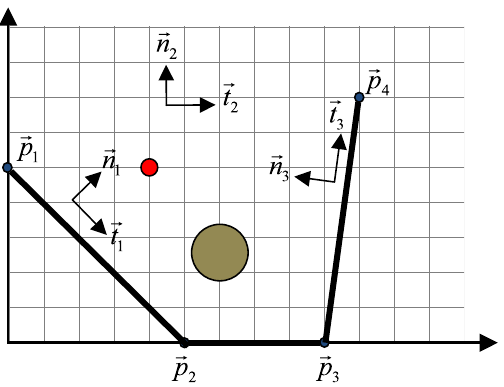
\includegraphics[width=0.8\linewidth]{./skizze_schieferFlipper}
	\caption{Skizze zum schiefen Flipper}
	\label{fig:1_skizze_schieferFlipper}
\end{figure}

\subsection{Gegebene Formeln und Konstanten}
Die begrenzenden Wände, durch Vektoren dargestellt definieren sich durch:
\begin{align}
\vec{p_1} = (0,5)^T \ 
\vec{p_2} = (5,0)^T \ 
\vec{p_3} = (9,0)^T \ 
\vec{p_4} = (10,7)^T
\end{align}

Die Position und der Umfang des zylindrischen Hindernisses entsprechen:
\begin{align}
\vec{p_Z} = (6,2.5)^T \ 
RHnd = 0.8
\end{align}

Startposition der Kugel
\begin{align}
\vec{xa}_{0} = (4,5)^T
\end{align}

Startgeschwindigkeit der Kugel
\begin{align}
\vec{v1}_{0} = (0,0)^T
\end{align}

Radius der Kugel
\begin{align}
R = 0.25
\end{align}

\subsection{Funktionen}
Im Folgenden werden die verwendeten MatLab-Funktionen dokumentiert.

\subsubsection{Init}
\begin{lstlisting}
function Init

% Hindernis und Pfosten fuer Waende
Hnd = [6;2.5];
p1 = [0;5];
p2 = [5;0];
p3 = [9;0];
p4 = [10;7];

% Kugel
x1 = [4;5];
v1 = [0;0];

% Normale und Tangentiale der Waende
t1 = (p2-p1) / norm(p2-p1);
n1 = [-t1(2,1); t1(1,1)];
t2 = (p3-p2) / norm(p3-p2);
n2 = [-t2(2,1) ; t2(1,1)];
t3 = (p4-p3) / norm(p4-p3);
n3 = [-t3(2,1) ; t3(1,1)];
\end{lstlisting}

\subsubsection{Acc}
\begin{lstlisting}
function [ax,ay] = Acc
ax = 0;
ay = -1;
\end{lstlisting}

\subsubsection{Wand1Refl}
\begin{lstlisting}
function Wand1Refl()

vt = v1' * t1;
vn = v1' * n1;

% Reflektierte Geschwindigkeit (mit Vektorisierung der Geschwindigkeit)
v1 = vt*t1 + (-vn*n1); 
\end{lstlisting}

\subsubsection{Wand2Refl}
\begin{lstlisting}
function Wand2Refl()

vt = v1' * t2;
vn = v1' * n2;

% Reflektierte Geschwindigkeit (mit Vektorisierung der Geschwindigkeit)
v1 = vt*t2 + (-vn*n2); 
\end{lstlisting}

\subsubsection{Wand3Refl}
\begin{lstlisting}
function Wand3Refl()

vt = v1' * t3;
vn = v1' * n3;

% Reflektierte Geschwindigkeit (mit Vektorisierung der Geschwindigkeit)
v1 = vt*t3 + (-vn*n3); 
\end{lstlisting}

\subsubsection{Wand1Kontakt}
\begin{lstlisting}
function kontakt = Wand1Kontakt
kontakt = (((x1-p1)' * n1) <= R);
\end{lstlisting}

\subsubsection{Wand2Kontakt}
\begin{lstlisting}
function kontakt = Wand2Kontakt
kontakt = ((x1-p2)' * n2) <= R;
\end{lstlisting}

\subsubsection{Wand3Kontakt}
\begin{lstlisting}
function kontakt = Wand3Kontakt
kontakt = ((x1-p3)' * n3) <= R;
\end{lstlisting}

\subsubsection{HndKontakt}
\begin{lstlisting}
function kontakt = HndKontakt
kontakt = norm(x1 - Hnd) <= RHnd + R;
\end{lstlisting}

\subsection{Stateflow-Modell}

Das folgende Modell veranschaulicht das Stateflow-Modell, das die Simulation durchführt.

Es gibt in diesem Modell nur einen Zustand, in dem erfährt die Kugel ihre Beschleunigung in Richtung \textit{unten}. Anschließend wird für jede Wand/Hindernis geprüft, ob die Kugel in Kontakt damit gekommen ist. Falls ja, dann wird berechnet in welche Richtung die Kugel umgelenkt wird.

\begin{figure}[H]
\centering
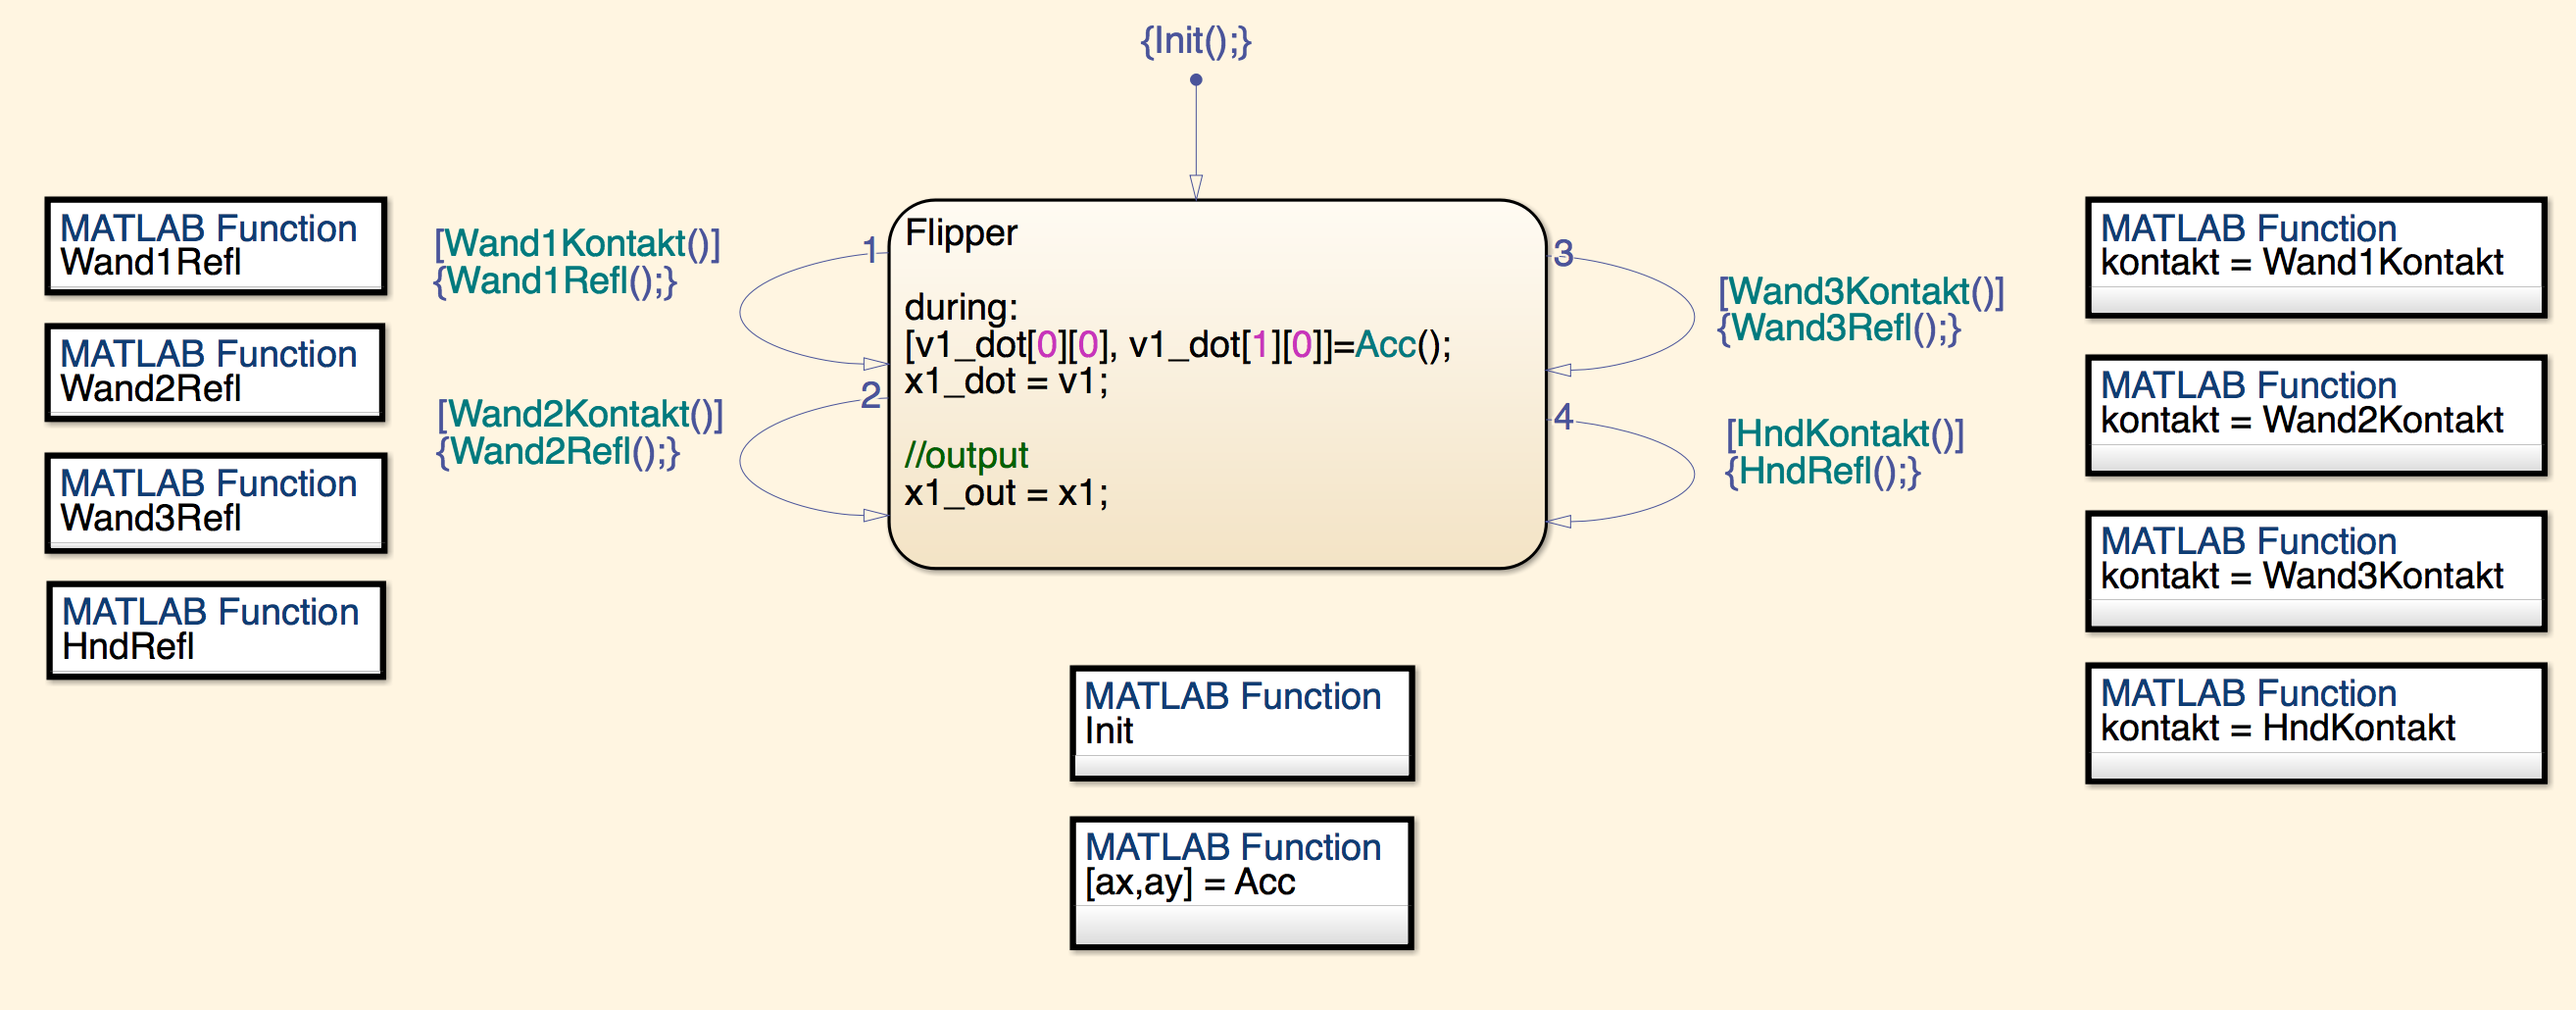
\includegraphics[width=1\linewidth]{./flipper_modell}
\caption{Stateflow Modell für den Flipper}
\label{fig:flipper_modell}
\end{figure}

\end{document}
